\documentclass[border=7pt]{standalone}

\usepackage{tikz}
%s\usepackage{tkz-euclide}
%\usepackage{amsmath}
\usepackage{amsfonts}
\usepackage{amssymb}


\newcommand\Mydiv[2]{%
$\strut#1$\kern.25em\smash{\raise.3ex\hbox{$\big)$}}$\mkern-8mu
        \overline{\enspace\strut#2}$}
\begin{document}
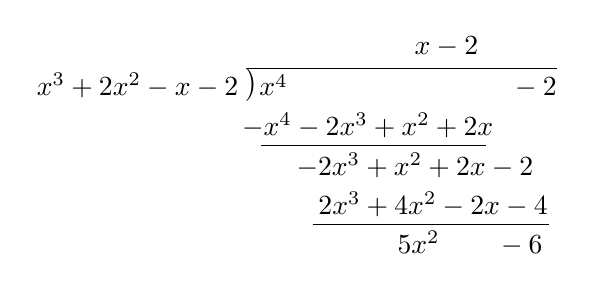
\begin{tikzpicture}

\node (c) at (0.5,3) {\Mydiv{x^3+2x^2-x-2}{x^4 \qquad \qquad \qquad \qquad -2}};
\node (c) at (1.4,2.5) {$-x^4-2x^3+x^2+2x$};
\draw (0.05, 2.25) -- (2.9,2.25);
\node (c) at (2,2) {$-2x^3+x^2+2x-2$};
\node (c) at (2.23,1.5) {$2x^3+4x^2-2x-4$};
\draw (0.7, 1.25) -- (3.7,1.25);
\node (c) at (2.7,1) {$5x^2 \qquad -6$};

\node (c) at (2.4,3.5) {$x-2$};



\end{tikzpicture}
\end{document}
